\documentclass{standalone}
\usepackage{tikz}
\usetikzlibrary{positioning, arrows}

\begin{document}

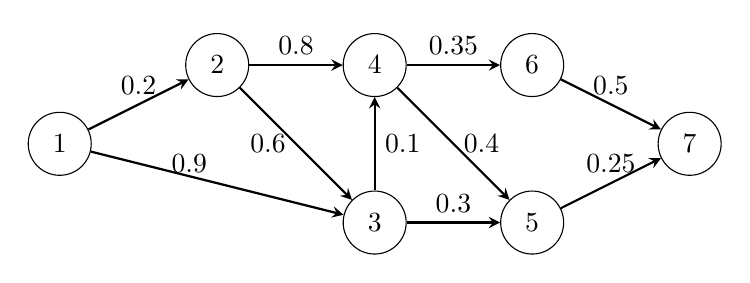
\begin{tikzpicture}[->, >=stealth, node distance=2cm, scale=1, transform shape]
    
    % Definir nodos con prefijo para evitar errores
    \node[circle, draw, minimum size=0.8cm] (n1) at (0,0) {1};
    \node[circle, draw, minimum size=0.8cm] (n2) at (2,1) {2};
    \node[circle, draw, minimum size=0.8cm] (n3) at (4,-1) {3};
    \node[circle, draw, minimum size=0.8cm] (n4) at (4,1) {4};
    \node[circle, draw, minimum size=0.8cm] (n5) at (6,-1) {5};
    \node[circle, draw, minimum size=0.8cm] (n6) at (6,1) {6};
    \node[circle, draw, minimum size=0.8cm] (n7) at (8,0) {7};
    
    % Definir aristas con pesos
    \path[draw, thick]
    (n1) edge node[above] {0.2} (n2)
    (n1) edge node[above left] {0.9} (n3)
    (n2) edge node[left] {0.6} (n3)
    (n2) edge node[above] {0.8} (n4)
    (n3) edge node[right] {0.1} (n4)
    (n3) edge node[above] {0.3} (n5)
    (n4) edge node[above] {0.35} (n6)
    (n4) edge node[right] {0.4} (n5)
    (n6) edge node[above] {0.5} (n7)
    (n5) edge node[above] {0.25} (n7);

\end{tikzpicture}

\end{document}
